\documentclass[10pt]{article}
\usepackage{amssymb}
\usepackage{lscape}
\usepackage[margin=.25in]{geometry}
\usepackage{fancyhdr}
\usepackage{multicol}
\usepackage{amsmath}
\usepackage{graphicx}
\usepackage{listings}
\usepackage{xcolor}
\usepackage{cancel}
\setlength\parindent{0pt}
\usepackage{adjustbox}
\usepackage[labelsep=quad, indention=10pt, position=bottom]{subfig}
\usepackage[latin1]{inputenc}
\pagestyle{fancy}
\lstset{
breaklines=true,
basicstyle=\tiny, %or \small or \footnotesize etc.
}
\begin{document}
\begin{landscape}
\begin{multicols*}{6}
\section{cis350 notes}
\tiny
Definition of software engineering: The application of a systematic dsciplined quantifiable approach to the development , operation and mtainenance of software. e.g. Tom takes 12 hrs, ben takes 8 hrs. how long to both paint \textbf{4.8 hrs}.
programming assumptions:  1) house tom and ben collected data on is the one they will paint (data collection of programmer output is inherently subjective). 2) homeowner wont change mind halfway thru painting (software requirements can and will change quickly). tom and ben have enough resources to never share it (shared software assets must be shared and maintained across multiple developers). 3) tom and ben will never do anything to slow each other down (never painting same thing twice, never going to pain another into a corner, ensuring most efficient. communication!) 4) no unforseen circumstances (what if market changes and product not needed) \textbf{biggest assumption is that there are no unexpeced mistakes}.
Programmers are bad at prediciting errors before they manifest. Software runs nearly every aspect of our lives and we know that software has been fault prone. software is custom built but errors can be hard to predict.
Engineering principles are \textbf{concepts rules or ideas to be kept in mind while solving an engineering problem}. no magic list, engineering principles are often earned thorugh mistakes and failures. principles can change in light of new challenges. SE is new and thus best principles are still being discovered. Bridge building example: they are becoming larger and more complex. Tacoma narrows bridge before collapse, builders thought lighter and narrower stuff was better for suspension. in the 1930s,aerodynaimics was poorly understood. forgot to consider vertical wind $\rightarrow$ destruction of tacoma narrows bridge.
Software princieples: use modern programming suites, when using 3rd party software, have contingency planes, ensure good modulaarizations, always document critical safety decisions. existing software is less risky than new custom software, use independent test teams when possible, code review can detect defts, always tes complete system within target environment .e.g gandhi bit overflow (-2 modifier to aggression normally, but when -1 overflows to 255 super agressive). modern compilers prevent this. heartbleed. navy social security leak. \textbf{Assessing risk} when you rely on third party software have risk assessment plan. should be identified and daddressed via \textit{avoidance, mitigation, having a contingency} esp w/regards to security. mars climate was lbs/sec vs newton/sec. NATS. old software can be costly (newer tech is cheaper and reduces error rates). as code ages, harder to maintain. \textbf{this is what software entropy is}. combatted with refactoring. \textbf{effort} refers to the time and money required to produce a piece of software. prediciting effort is diffficult. effort estimation resesarch provides models to predict time and cost of softare production. most use historical data and have wide margin of error. Therac-25 (no indep code review, unhelpful error messages, not testing with hardware and software together until in hospital). \textbf{importance of testing} is the best way to catch software ffailure is to find it in testing, can never be exhaustive, should mimic the end enviorment as much as possible, code reviews are often encouraged in conjucntion with testing. nothing caused by malicious intent. no criminal mastermind. well intentioned programmers who made mistakes, didn't check thoroughly and didn't assess risk. \textbf{learn why did faulure accur, what was the risk and how it could have been avoided, what can we change so it never happens again}.
SE is about developing and utilizing engineering principles to produce software, learning from mistakes and enactivng systemic change to avoid or mitigate risk. SE concerned with \textit{process over product, tools to help with software development, improving development efficiency}.
\textbf{LECTURE 2}
Standish Group CHAOS Report 1995:
16.2\%of software projects are successful: On time, on budget;
52.7\% of software challenged: Over budget and/or over time, Fewer features than specified;
31.1\%Failure;
189 percent initial cost. twice as long as expected. only 61 percent of features
Properties of good software: work as speicifed, does what the customer asked for, stable/predictable (bug free), maintainable, cost effecitve.
Six major steps of software: specification, design, development, testing, deployment, maintianance. \textbf{ad-hoc} building and fix, cowboy coding: 1) build first version 2) modify until customer is happy.
Software life cycle models: constructs that dictate life cycles models. disclaimer, no one adheres to a model perffectly and hybrid models exist.
Waterfall theory: each phase (req gathering, system design, implementation,testing, deployment, maintiance) falls into the next (e.g. fully complete requirements and design before any code is written, no new features after coding starts). Simple model, easy to manage, clear deliverables, process don't overlap. disadvantage of series design flaws may not be discovered until testing, no working code until late in the model. immobile to requirement changes. Iterative waterfall model: overcomes some of the inflixibility of waterfall, but going back phases is expensive and time consuming, should be avoided.
Incremental model: build 1,2,3. build on a system incrementally (consumers get to see product as it is conconstructed). doesn't offset need for heavy planning at the beginning. more expensive than waterfall. problems with earlier versions can arise later.
Iterative prototyping: building prodtotypes of efeatures get short term feedbacks in gaming. Protypes are vertical (fully demonstrates small subset of features, lacks features not shown completely) or horizontal (show overview of system, ui prototypes are great examples).
Different types of prototypes: throwaway (costly but prevents long term instability, evolutionary reduces long term cost, but less mtaintainbable, incremental, extreme.
Incremental vs iterative (incremental is parts of mona lisa painting, iterative is outlines and filling it in further and further).
Agile isn't a method: it is a collection of methods that fits the agile manifesto. Individuals and interactions over Processes and tools Working software over Comprehensive documentation Customer collaboration over Contract negotiation Responding to change over Following a plan
That is, while there is value in the items on the right, we value the items on the left more.
Scrum: product backlog, sprint backlong, 2-4 week period (24 hrs  scrum), potentially shippable product increment. Short, information-based, not problem-solving (problem solving and questions offline after meeting). Three questions: what did I accomplish yesterday? what will i do today? what obstacles are impeding my progress?
Benefits of agile: open to design changes. response to requirements changes more easily than planned methods. large amount of face to face tim. incremental releases keep customers informed and happy. fixed time scales of relases. has a better track record in code quality and speed of development. disadvantages: collaboration is time consumeing. requires heavy coustomer interatction, evolving requirements mak prdicting effort difficult, scalability concerns, code  quality can degrade over srpints, turnove.r BEST APPROACH IS AGILE. LEAN IS NOT AN ALTERNATIVE TO AGILE (about learning eliminating waste).
\textbf{Requirements engineering} (hardest thing is deciding what to build). cost of change increases over time. Two types: HIGH LEVEL (business requirements); what benefits will cust. cget and users get. LOW LEVEL: what will system do, how well?
Steps: Find problem to solve, do concept exploration to determine if software is a good solution, determine a set of requirements to solve the problem, specifiy the requireements specifically, validate requirements.
Goals: defint the problem, explore constraints, understand operation environment, address high level details of solution. determine feasibility \textbf{3 questions to ask} shoud system be built, must it be built,can it be built. should it be built (is problem important, how frequent is the porblem, is the market for the problem large enough to justify the cost, would automated solution be better). must a system be built (is the solution already out there). can a system be built (what is the feasibility, two types: technical and political e.g. workforce, management, finances, laws). Cost benefit analysis are there resources. feasibility is fin flux. technology improves, companies change. \textbf{requirements engineeringp rocess: elicitation, specification, validation}. elicityation: find a consumer with problem, get list of requirements. asking what you want doesn't work, need specifics. stakeholders don't know anything, devs may not understand system requirements, diff stakeholders describe same thing different ways. reqs change. INTERVIEW (close interviews, open interviews, jargon heavy, obvious info not obvious, avoid preconceived ideas about the software. visual prototypes for interfaces), ETHANOGRAPHY (observe day to day stifels innovation), user stories (process by which a task will be completed or used, narrative). Scenarios: initial assumption, description of natural flow of events. description of what can go wrong, other activities, description of end result.
User story guidelines: e.g. as a student user, i can create a new question and specify the folders, summary, an details. needs to be discrete but not precise, estimable (possible to estimate work needed), traceable (possible to know which parts of system satisfy the requirement), testable(so you know its done). \textbf{requirements are features, function, capability, property a software product must have and it must be testable!}. eliciting requirements by close ended (specific and detailed), open ended, scenario (lets customer talk thru seq. of interactions), and probing (forces customer to think about justification for each requirmeents). requirements spec is much more specific than concept exploration, concept exploration determines what software CAN do, req specs are what software will do.
2 stakeholders, user requs (consumer), system reqs(developer). User Requirements are requirements designed
for review by end user, but may often lack details. Use broad statements to convey intent. These have to be turned into System Requirements. System Requirement high detailed list of requirements for a system.
Functional: Describe the services/ features/ operation of the system. (user should be able to search for all clinics. system wil lgenerate daily report listing all appointmentso f the day)
Non-functional: Constraints under which the system operations (user should be able to use after 1 hr of training. list should load within 0.5 s)
Godo requirmeents: complete, testable, traceable, consistent, concise, readable, feasible, changeable
What is good software: ISO 9126: functionality (satisfies needs), reliable (correctly operates), usability (effort eneded to use software), efficiency, relation between performance and amount of resources, portability (can be transfered from 1 env to another). Internal quality of maintainability (can be uderstood), changeability (can be asily modified), stability, and testability. \textbf{how to we achieve internal quality} DESIGN.
What is system modeling: process of developing abstract models of a system. each abstract model presents a different view of that system. system modeling often involves diagramming interaction and processes. system model isn't complete rep of system, it is an abstraction not a translation. Can be used during design, implementaiton, and after implementation. external perspective is to model the content or environment of the system and how it gets used by the user. interaction between system and environment... \textbf{structural} model the organization of system and data, \textbf{behavioral} model the dynamic behavior of system and how it responds to events.
UML diagrams (unified modeling language). activity diagrams show all activities in process. use case diagrams show interactions between system and environment. state diagrams show how system reacts to events. class diagrams show object classes and realtionship. sequence diagram shows interactions between actors and complenets in the system. 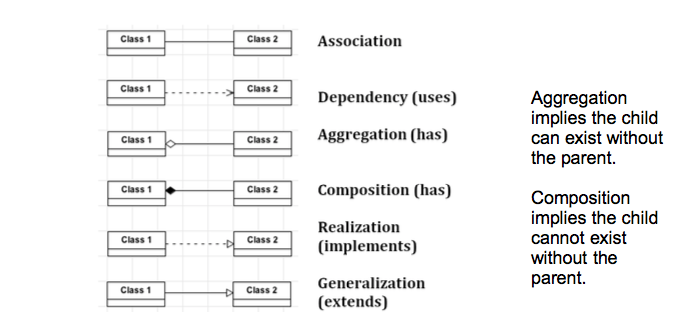
\includegraphics[width=\columnwidth]{uml}
SOFTWARE DESIGN:
Essential difficulties: complexity: software not buiilt on repeatable parts, building two pieces of software not like building 2 cares. complexitiy is inherent to software. no one person will fully understand an entire system \textbf{conceptual integirty} (many people agreeing on understanding) is impossible.
Conformity: software must integrate with different interfaces, users, systems, requires more complexity
Changeability: infinitely malleable. manufactured things are rarely changed after manufacturing (in software however change is the norm). New users discover product, pushing edge chases. changing tech also creates change.
Invisibility: we can have several different diagrams mapping the same system, overlaying graphs would be complicated.
How do we organize code \textbf{modularity, functional independence} and how should we expose functionality (\textbf{abstraction, information hiding}).
Technical debt is the cost of poor deisgn decisions becomes worse over time. a form of delayed gratification, only for whatever the opposite of gratification is ``delayed screwing yourself". Lack of documentation or changeability.
Incremental changes is the repeated process of adding to code base. used in development by adding new features, expanding or improving existing features. maintenance fixing ffedfects reducing technical debt.
Incremental change process (before writing code). initiation (analyze user stores and change requirements and extract concepts). concept location is locating concepts in the source code. impact analysis is the set of classes/methods likely to be affected by teh change. prefactoring is to refactor to make changes easier. DURING THE CODE actualization is the ipmlementation by writing new code and incorporating it into the system. propagation is to propagete the changes thru the system. post factoring, new baseline is toe commit the changes.
Modularity. split stuff up (Tweet class stores records and calls TweetFinder and TweeetTime). UNDERSTAND THE ASSUMPTIONS YOUR INTERFACE MAKES. \textbf{single responsibility principle} each module should only have one reason to change. should only address 1 part of the requirements. cohesion: all functionality should be closely related, breaking into smaller modules is gooood.
Functional indepdence. example: if i find the tweet within the tweet module i have to know a lot about the state. if i have a separate module i only need to know about the interface. Loose coupling good, tight compling bad (requires more info than needed, modules depend on each other and share global data).
Abstraction is to program an interface. what they do not how they do it. have functions input output based. Abstract data types (just need a list, doesn't matter what). things to avoid. THE GOD CLASS
Architectural patterns: Pattern is a way of presenting, sharing, and reusing knowledge about a software system. a pattern is an architectural pattern is an abstract description of good practice with the pattern. this good practice description comes from yeears of experiences. this description clearly identify if pattern is appropriate and where it isn't. details advantages and disadvantages. \textbf{monolithic} single module or small number of tightly coupled modules, simple to develop/scale/deploy. larger code base is intimidating, difficult to learn, and dev is difficult. \textbf{component based} is the collection of off the  shelf moduels that provide various services. these modules are glued together. having multiple components in the same view is difficult. \textbf{client-server} system is presented as a set of services. service is represented by a separate server. multiple clients access each server to use the service. service access backend data structure. some network is used to access these services. used when data in shared db needs to be accessed from multiple locations and if the load on the system is variable. allws for dist of services across network. general functiaonities can be available to add clients and doesn't need to be implemented on all services. individiauls services can be modified independently. disadvatnages. limited by network and unpredictable (security stuff also). \textbf{software as a service} client-server + component based. growing use of web based interfaces makes the market potentially large and system agnostic. all problems of web dev. \textbf{MVC} Model view controller. model manages data. view manages information for the user. controller manages user interactions. separates presentation and interaction from data. 3 models interact to control, view, and manupulate data. allow multiple ways to view data, useful when requirements are unknown. Advnatages allow the data to be indep of the representation. supports using data in dif ways. disad: means more code though. \textbf{layered architechture} has presentation layer (UI), application service/interface layer (ui management), business logic layer that enforces real world limitations on data, data access layer interface with db, and system later OS interfaces. In theory same separation and indep of MVC, can change each layer without changing other ones. users are the top, low level bottom. interactions have to travel up and down a layer. use when building on otp of existing system of services or data (good for dist dev as each team can work on a layer, good for sec). advantage is replacement of layers, redundant actions are in all layer. disadvantage is that making diff between layers is hard, interface pass thru is hard. requirements changes may be needed. more code.
public class StudentMVCDemo \{
public static void main(String[] args) \{
Student model  = retriveStudentFromDatabase();
StudentView view = new StudentView();
StudentController controller = new StudentController(model, view);
controller.updateView();
controller.setStudentName("John");
controller.updateView();
\}
private static Student retriveStudentFromDatabase()\{
Student student = new Student();
student.setName("Robert");
student.setNumber(10);
return student;
\}
\}
\textbf{Groups of design patterns}
Creation patterns: handle obejct creation and instantiation. Structural patterns bring existing objects together. behavioral patterns give a way to manifest flexible behavior. \textbf{Iterators} allow you to visit all elements of a collection one at a time. if you implement a collection, must have iterator. has functional independence and information hiding (don't have to know how collection is structured, just need to know if it works) it is a MEME. Creational patterns used that hide or limit constructor usage. Singleton: only one instance at a single time. that instance can be shared across multiple modules (e.g. logger). never use singleton if you need multiple. \textbf{Factory pattern} is when you might need to use a class on the flight by combining existing pieces. Interchagable pieces of a system and put them together! Abstract factory pattern, having indepdent factories is bad. more classes = more complexity so the solution is to build several factories where the programmer can ``order" the class they want. have all the factories share an interaface so ordering is simple.
// SINGLETON
public class Logger \{
private static BufferedWriter logWriter;
private static Logger instance;
private Logger()\{
logWriter = new BufferedWriter(new FileWriter("log.txt"));
\}
public static Logger getInstance()\{
if (instance == null) \{
instance = new Logger();
\}
return instance;
\}
public void writeToLogFile(String s) \{
\}
\}
public class SomeOtherClass \{
public static void logExample()\{
Logger log = Logger.getInstance();
log.writeToLogFile("Inside some other class");
\}
\}
// ABSTRACT FACTORY
public abstract class AbstractFactory \{
abstract Color getColor(String colorType);
abstract Shape getShape(String shapeType);
\}
public class AbstractFactoryDemo\{
public static void main(String[] args) \{
AbstractFactory shapeFactory = FactoryProducer.getFactory("SHAPE");
Shape shape1 = shapeFactory.getShape("CIRCLE");
shape1.draw();
Shape shape2 = shapeFactory.getShape("RECTANGLE");
shape2.draw();
AbstractFactory colorFactory = FactoryProducer.getFactory("COLOR");
Color color1 = colorFactory.getColor("RED");
color1.fill();
Color color2 = colorFactory.getColor("BLUE");
color2.fill();
\}
\}
Bridge pattern is decoupling an abstraction from its implementation so that the two can vary indepdently. maintain spearate inheritance hierarchies that ally a client to assumble combinations as needed. have an abstract implmentor that selects a concrete implmentor. Shapes.
List
<Shape>
shapes = . . .
shapes.add(new Circle(50, 50, 20, new GrayscaleRenderer());
shapes.add(new Rectangle(80,80,120,120,
new ColorRenderer());
for (Shape s : shapes)
s.draw(); // use the interface
interface Renderer \{
Void drawCircle(int x, int y, int radius); Void drawRectangle(int x1, int x2,
int y1, int y2);
\} class ColorRenderer implements Renderer \{
. . . \}
class GrayscaleRenderer implements Renderer \{
. . . \}
// DECORATOR
abstract class Ingredient implements Drinkable\{
protected Drinkable base; public Ingredient(Drinkable b) \{
base = b;\}
double price \{return base.price();\} String toString \{
return base.toString();\}
\}
bid ball of mud is software that lacks clear structure or architecture. system are appended haphazardly and expeditiously. internal software qual deteriorates. God class sucks.
Review: Creational Patterns handle object creation and instantiation Singleton - only one instance can exist at a time, shared by multiple modules without those modules being aware of each other Factory - defer instantiation to subclass, define interface for creating object, but let subclasses decide which class to instantiate Abstract Factory - have several factories share interface to make 'ordering' simple. Structural Patterns bring existing objects together Bridge maintain separate inheritance hierarchies that ally a client to assemble combinations as needed, abstract 'implementer' selects a concrete implementer Decorator on the fly object creation Adaptor adapt existing class/object to new interface without changing underlying class (useful to update interfaces while minimizing side effects/propagation of changes) Facade hide a complicated interface or set of interfaces with a single interface (useful to hide complex interfaces that are hard to use correctly). Behavioral Patterns give a way to manifest flexible behavior Iterator allow you to visit all elements of collections one at a time, functional independence, information hiding Observer Objects need to notify varying list of objects that some event has occurred (variable change method called), possible that you'll want to link objects to notify each other at runtime Strategy class that represents the strategy and pass instance to method that implements rest of algorithm

PORTABILITY:
software portability is the usability of software across multiple systems, interfaces, architectures, platforms, etc. most of the market is android. Most of the time spent consuming media is now on mobile. gaming on mobile has now increased beyond dedicated systems. WHY DO WE NEED PORTABILITY? hardware and software come and go "things change, people change, hairstyles change, interest rates fluctuate" software you write for a target system may outlive the target system. even the basic paradigms of how you write and use software changes overtime. WHY DO WE STILL USE OLD SOFTWARE? new software is significantly more expensive to produce, cheaper to port existing software. COBOL: inertia is a strong force, the cost of rewriting cobol is too prohibitive and replacing everything is also prohibitive and risk-intensive. demand for cobol programs to interface with legacy systems. we have a lot of new platforms, people use different devices and each has its own architecture. Windows can't run linux bc executable architecture of windows is different from linux. Linux uses ELF (executable and linkable format), Windows uses PE (portable executable). Porting from iphone -> android (iphone uses obj c, android java). porting reqs full recoding or web-based apps. both limited c useage but android has limited c api. have different styles, iphone doesn't have native back, android does. WAYS TO PORT SOFTWARE independent development on native platforms, pros: application optimized for each platform. cons: significantly more effort, new feats need to be implemented twice, diff bugs may emerge on diff systems. OR use high level lang to compile on diff systems, take src and build on each system. pros: code once build twice, cons: reqs access to both systems, system specific probslems may arise. Common solution: core functionality in C++, interface modules are programmed separately for each interface. 3-Tier/Layered: Presentation tier <-> Application Tier <-> Database Tier. Can also cross compile: compile on one host system for all other systems (designing apps for android on windows). easier when dealing w/large num of platforms. costs: requires cross compilers, bugs on tgt systems have to be fixed. costly/time-consuming debugging. more than making software work. cultural and non functional differences. Windows 9 not exist bc bad code. also windows v linux: linux likes having cmd lin whereas windows pref gui.

USABILITY
Why use real world examples? b/c bumans compare a computer interface to real world interface. Software quality IOS 9126: INTERNAL: analyzability, changeability, stability, testability. EXTERNAL: functionality, reliability, efficiency, usability, portability. WHY IS USABILITY IMPORTANT? Therac-25. Radiation therapy machine involved w/6 accidents b/w 1985-87. moved some safety features from hardware to software. some software from therac-20 was used and assumed to be correct. safety analysis, assume software would be tested extensively and did not allow for possibility of residual errors. Hamilton, Ontario, Jul 1985. Machine stopped 'no dose', common occurrence, technician pressed "p" to proceed, re-delivers' dose. happens 4 more times. patient gets 5x more dose, died 4 mnths later. Tyler tx 86. delivered 1 x dose of radiation. also typer tx, malfunction 54 = death. WHAT MAKES SOFTWARE USABLE? 5 Es: Effective- can accomplish a task, Efficient- can accomplish task quickly w/minimal user effort. engaging- user wants to learn the interface, easy to learn- initially or over time. error tolerant- able to recover from user errors. Intuitive...bc not everyone has equal experience. DESIGNING FOR USABILITY: USER CENTERED DESIGN: Persona: who are the users/ what do they know, what is their motivation. SCENARIO: what do they want to do? what are the doing/thinking? what are their expectations of the system? INFORMATION VISUALIZATIONS: part of dev of user interfaces w/how info is represented. comp sci + cog psyc. HUMAN PROCESSOR MODEL perception pipeline. senses => perceptual subsystem -> visual/auditory image storage -> working memory <-> long term memory -> cognitive processor OR motor processor -> movement response. Perceptual, cognitive, and motor subsystems. INFO VIZ: METAPHORS: metaphor = socially agreed upon construct that relate to importance and significance. In info viz, metaphors are used to indicate which data is more important and attract users eyes to appropriate place. EVALUATING USABILITY: HEURISTICS: general guidelines or widely accepted best practices, USABILITY STUDIES: observe ppl using the system under normal circumstances. METRICS: measure quantitative aspects such as time to complete task, error rate, memorability. NIELSEN USABILITY HEURISTICS: 1. Match b/w system and real world 2. consistency and standards 3. Help and documentation 4. user control and freedom. 5. Visibility of system status. 6. Flexibility and efficiency of use. 7. Error prevention 8. Recognition rather than recall. 9. Recognize/diagnose errors 10. aesthetic and minimalist design. Usability studies: Focus groups (few ppl), surveys (many), Observation (few doing in controlled setting), ethanography (many doing field obs in nat setting). USER METRICS: HUMAN RELIABILITY ASSESSMENT: error rate - how often mistake, cognitive load - how much does user keep in their mind during a task. memorability -how much does the user remember  What makes usability important -> therac-25. what makes it usable? 5Es, how do you make usable software? user-centered design. Info vis? metaphors. Evaluating usability: Heuristics, studies, metrics. INTEGRATION: what order do we implement our systems in? consider hw1. userInterface -uses -> processer - uses -> TweetReader. TweetFileReader Implements TweetReader. Everything uses Tweet, User Interface has a processor. processor has a tweetreader. tweetreader is extended by tweetFileReader. WHAT BROAD STRATEGIES CAN WE IMPLEMENT? BIG BANG INTEGRATION: integrate all components as they are completed. BOTTOM UP INTEGRATION: implement and test modules without dependencies, then implement things that only depend on implemented things. TOP DOWN INTEGRATION. Implement and test moduels on which nothing depends. Then imepelment and test modules on which nothing unimplemented depends. BIG BANG - >basically ad hoc. can lead to "integration hell", code may not even compile without significant interface. Difficult to test. If the output is incorrect, which system or tier is responsible? BOTTOM UP: Write TweetFileReader first. Advantages: do developement and integration together, clearer indication of responsibility errors. Disadvantages: Assumes no cyclic dependencies, design is completely planned out. lowest level modules are easy to implement/test. If implementation finds necessary design changes, this can be time consuming. TOP DOWN: First implement UserInterface. Use STUBS to simulate dependencies. Advantges: tested product is consistent because testing is performed basically in the end environment, stubs are quick and easy to write. STUB EXAMPLE: String state = getState(); List<Tweet> result = processor.getTweetsForState(state); for (Tweet tweet : result) \{ system.out.println(tweet) \} . We don't have to implement Processor.geTweetsForState(state); before testing the UI. What that woud look like: List<Tweet> getTweetsForState(String state) \{ List<Tweet> tweets = new ArrayList<Tweet>(); tweets.add(new Tweet(...)); ... add dummy data; return tweets; \}. THE GOAL OF A STUB: stimulate just enough functionality so that other modules can be tested. Write stubs when stubs are simpler than underlying processes. POJOs: Plain Old Java Objects; Technically a subset of javabeans with fewer results. Generally a collection of data + getters/settiers.  Doesn't do things, just stores things. There are easier to impelemnted than write stubs for so we just impelement them . TOP DOWN INTEGRATION CONTINUED: we've implemented user interface using "Processor" that is all stubs. No we impelement Processor, suing stubs for its dependences (Tweet Reader). HOW SHOULD WE CREATE DEPENDENCIES? Option \#1: hardcode them: In UiserInterface. TweetReader tr = new TweetFileReader(); Option \# 2: let client create them. Processor processor = new Processer (new TweetFileReader()); Option \# 3: factory method pattern: Processor process = new TweetFileProcessor() // a factory that generates a processor, which is given TweetFileReader(); Option \# 4: Singleton Pattern. TweetReader tr = TweetFileReader.getInstance(); SOFTWARE TESTING: Bridge testing, less obvious when software fails. Intention plays a big role in whether or not software is "correct' correctness is domain specific. Intention plays a big role in whetehr or not software is correct. correctness is domain specific. How did you know you program worked? How do you know the tournament you generated was the best one? You'll never know if your code is correct. Event trivial software can have theoretically infinite input. cannot test all input. Testing CANNOT prove code is correc.t SOFTWARE TESTING: Executing a piece of software with intention of finding defects/faults/bugs. SOFTWARE TESTING: Software testing is intended to ensure the program behaves correctly. Testing is useful for discovering defects before delivery. Testing typically involves executing a program artificially. If you want to test a bridge you fail. However, software can be hard to test because. 1) Demonstrate to the developer and customer that the software meets requirement, for generic software one test for each system feature included in release: This is valled validation testing. Two goals of software testing; detects inputs or seq of input to create errors (defect testing). Validation: did we do it right? Defect: how broken is it? Testing: can only show presence of errors, not their absense. Exhaustive Testing: attempt a test w/every possible input. Radom Testing: select random inputs. Black-box testing: select inputs based on specific space. CONTROLLABILITY: easy to put into a state that you want to test. OBSERVABILITY: easy to observe external behavior of a system. EQUIVALENCE PARITIONING: Assume similar inputs behavior similarly. divide the sapce of inputs into smaller grousp and pick a representative exmaple. ROBUSTNESS TESTING: inputs that are syntactically valid but semantically not meaningful: Test error handling. BOUNDARY CONDITIONS: Look for inputs on the boudaries b/w two equivalence classes. WHITE BOX TESTING: statement coverage: hazve at least one test covering every statement, condition coverage: have every boolean eval to both tru and false, BRANCH COVERAGE: for every if do you eval to t/f? for every look, do u eval normal iter, one pass, zero passes, infinit condits? Code is a graph, you want to cover every node and every edge w/one test. WILLOW TREE: Prod strat -> design -> architectural prep -> dev \& QA -> launch. Prod strat: UX Strate (what to build), id business obj user centric approach (user interviews, personas, surveys, ethnographic research). Architecture, What can be built? client landscape. Product design: look and feel branding usability. Architecture: How it should be implemented, class org, coding style, api access, inheritance vs composition. Analytics: g o thru each screen, find key uses, AB testing, collect lack of data. Dev: break down features, est tickets, sprint planning. QA: qual assurance, make sure the app works, dev test scenarios. Launch \& Live support. Commenting: gets out of date, hard to maintain, diff writing styles. Imp. complex code, somtimes hack necessary. magin nums. self doc code: variable names, method names, easy to read, you see exactly what the code is doing, up to date. SOURCE CONTROL: Git af. Continuous integration: centralized certs, consist. build env, improve workflow, async build process, id testing errors for review. CodeReview be open, learning, never be afraid to share. TESTING: test first, code later, forsee problems, outline diff scenarios. help rethink impl. unit tests: any logic in the app, API calls, Model View Viewmodel, UI Tests, Reactor. Smoke tests. Overcommunicate. READABILITY: you'll read your code far more times than you will write it. you won't remmeber when you were thinking when you wrote the code. other will have to read your code, readbility and understandability matter. READABILITU: ease that readers can id and differentate tokens and syntactic meaning. UNDERSTANDABILITY: ease with which a reader can identify the semantic meaning of code. READABILITY: syntactic meaning: whitespace usage, spacing and indentation, identifier length, use of dictionary words, variation b/w identifiers. UNERSTABILITY: necessary but not sufficient for understabile code to be reasonable. code has to be readable to be understandable, but readable code isn't necessarily understandable. Comments, adherence to coding conventions? meaningful identifier names, unambiguous including units of measure. Strucutral: \# of paths thru code (too many = bad for understandability) \# of identifiers: \# of identifiers needs to be as small as possible.

TEST DRIVEN DEVELOPMENT AND DEFENSIVE PROGRAMMING: Test driven development- write the black-box tests first, before writing code. implement just enough code to make the tests pass. if your method still requires new features, write more tests that fail and then repeat.DEFENSIVE PROGRAMMING: writing your code in such a way that it cannot be used incorrectly. Strategies: Don't do anything unique: bad in -> bad out. Notify caller: bad in -> error. Halt: bad in -> stop. Error codes are bad bc they aren't meaningful, not possible, and easy to ignore. Exceptions force the caller to handle the error by throwing exceptions. These are preconditions, things that we assume to be true at the start of the method. Difficulty in just having a "catch all" Exception and doing nothing. Assert will throw an assertion error (things that should never happen). JVMs disable assertion errors and may appear in dev but not deployment. Post conditions: thats that should be true at the end of the method. what to do? Option 1: ignore and let the caller deal with it. Option 2: roll back and notify (undo any changes and throw exception). Roll back bc if the exception is caught and handled the state must be assumed not to have changed. Option 3: Halt (assert False). FINISHING UP TESTING + EFFICIENCY: bug reports: ID and describe an encourtered defect, provide means by which the bug can be reproduced, identify expected behavior, severity of the bug, workarounds. Format: title, actions performed, expected vs actual results, environ. Stack trace gives u a snapshot of the program when it creashed associated with the trace sometimes. print statements are bad and assumes you have somewhere to print. Debuggers: get familiar with them (variable watches, breakpoints, step into vs step over vs step return vs reusme). Advntages: see all the variables, not just you print. you can watch the state of the program change after each step. you don't have to make any code chagnes. Debug model imitations: significant cost, where to breakpoint isn't easy, no backtracking. debug can tell you that a variable is null but not why. EFFICIENCY: Rule 1: USE THE RIGHT DATA STRUCTURE AND ALGORITHM: arraylist vs linkedlist not equal. hashing saves a ton of time. Know Linkedlist, arraylist (always better), vector(arraylist with synchronization). Sets: TreeSet is a balanced BST, HashSet uses hashing. HashMap also. Need duplicates -> lists. Order? Lists or treesets. Any other time: sets. LAZINESS dont do it until you actually have to. SHORT CIRCUITING: Use power of short circuiting to your advantge, execute in order of complexity. MEMOIZATION: Trade off b/w space \& time complexity. LazyInitiation: don't instantiate until method call.

PARALLEL
Embarrasingly Parallel: Something that is incredibly easy to make parallel. Example from class: applying an image filter line by line. "COST" OF THREADS: defined as CP(n) = p * TP(n), where p is the number of processors, T the processing time and n the input. Starting threads has a time value that could make parallelizing beyond a point ineffecient. CREATING THREADS Threads can be created through implementing runnable, which loosely couples with your choice of concurrency or through extending thread, which forces concurrency. Callable adds the ability to return results and also throw checked exceptions. Run executes a thread. Start because a Thread.JVM and calls the run method. Join waits for a thread to die, can specify time in milliseconds. Interrupt interrupts a thread Some methods that block such as Object.wait() may consume the interrupted status immediately and throw an appropriate exception (usually InterruptedException). Stop stops a thread and is deprecated. EXECUTORS Executors abstract the low-level details of how to manage threads. They deal with issues such as creating the thread objects, maintaining a pool of threads, controlling the number of threads are running, and graceful / less that graceful shutdown. SYNCHRONIZATION The synchronized keyword is all about different threads reading and writing to the same variables, objects and resources. CRITICAL SECTION are things that need to be synchronized. However, global things should not be synchronized. Strings should also not be synchronized since all strings with the same value will be synchronized due to how Java is built. However, THREAD HANDLING is best done by synchronizing classes that handle variables that multiple threads may be attempting to access. This is done through the synchronized keyword.

\end{multicols*}
\end{landscape}
\end{document}
